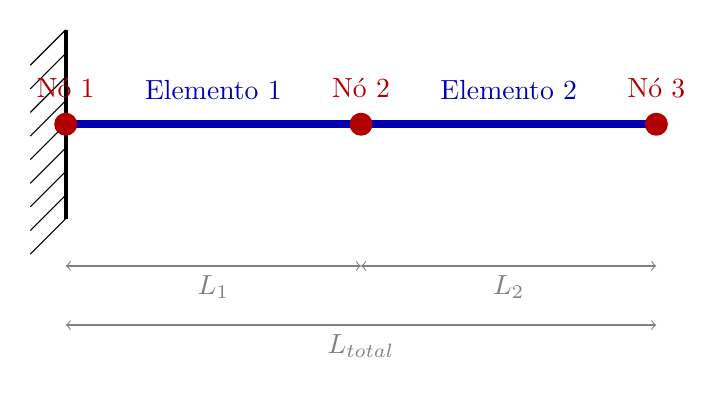
\begin{tikzpicture}[scale=1.5, thick]
    % Coordenadas dos Nós
    \coordinate (N1) at (0,0);
    \coordinate (N2) at (2.5,0);
    \coordinate (N3) at (5,0);

    % Engaste na esquerda (Nó 1)
    \draw[line width=1.5pt] (0,-0.8) -- (0,0.8);
    \foreach \y in {-0.8,-0.6,...,0.8}
        \draw[thin] (0,\y) -- (-0.3,\y-0.3);

    % Elementos Finitos da Viga
    \draw[line width=3pt, blue!70!black] (N1) -- (N2) node[midway, above=4pt] {Elemento 1};
    \draw[line width=3pt, blue!70!black] (N2) -- (N3) node[midway, above=4pt] {Elemento 2};

    % Nós e Rótulos dos Nós
    \filldraw[red!70!black] (N1) circle (2.5pt) node[above=6pt] {Nó 1};
    \filldraw[red!70!black] (N2) circle (2.5pt) node[above=6pt] {Nó 2};
    \filldraw[red!70!black] (N3) circle (2.5pt) node[above=6pt] {Nó 3};

    % Linhas de cota e comprimentos
    \draw[<->, thin, gray] (0,-1.2) -- (2.5,-1.2) node[midway, below] {$L_1$};
    \draw[<->, thin, gray] (2.5,-1.2) -- (5,-1.2) node[midway, below] {$L_2$};
    \draw[<->, thin, gray] (0,-1.7) -- (5,-1.7) node[midway, below] {$L_{total}$};
\end{tikzpicture}